\documentclass{article}
\usepackage{fullpage,amssymb,amsmath,epsf}
\usepackage[12pt]{extsizes}
\usepackage{psfrag}
\usepackage{graphicx}
\usepackage{enumerate}

\newcommand{\loss}{\mathsf{L}}

\newcommand{\newsec}{\section}
\newcommand{\denselist}{\itemsep 0pt\partopsep 0pt}
\newcommand{\bitem}{\begin{itemize}\denselist}
\newcommand{\eitem}{\end{itemize}}
\newcommand{\benum}{\begin{enumerate}\denselist}
\newcommand{\eenum}{\end{enumerate}}

\newcommand{\fig}[1]{\private{\begin{center}
{\Large\bf ({#1})}
\end{center}}}

\newcommand{\cpsf}[1]{{\centerline{\psfig{#1}}}}
\newcommand{\mytitle}[1]{\centerline{\LARGE\bf #1}}

\newcommand{\myw}{{\bf w}}

\newcommand{\mypar}[1]{\vspace{1ex}\noindent{\bf {#1}}}

\def\thmcolon{\hspace{-.85em} {\bf :} }

\newtheorem{THEOREM}{Theorem}[section]
\newenvironment{theorem}{\begin{THEOREM} \thmcolon }%
                        {\end{THEOREM}}
\newtheorem{LEMMA}[THEOREM]{Lemma}
\newenvironment{lemma}{\begin{LEMMA} \thmcolon }%
                      {\end{LEMMA}}
\newtheorem{COROLLARY}[THEOREM]{Corollary}
\newenvironment{corollary}{\begin{COROLLARY} \thmcolon }%
                          {\end{COROLLARY}}
\newtheorem{PROPOSITION}[THEOREM]{Proposition}
\newenvironment{proposition}{\begin{PROPOSITION} \thmcolon }%
                            {\end{PROPOSITION}}
\newtheorem{DEFINITION}[THEOREM]{Definition}
\newenvironment{definition}{\begin{DEFINITION} \thmcolon \rm}%
                            {\end{DEFINITION}}
\newtheorem{CLAIM}[THEOREM]{Claim}
\newenvironment{claim}{\begin{CLAIM} \thmcolon \rm}%
                            {\end{CLAIM}}
\newtheorem{EXAMPLE}[THEOREM]{Example}
\newenvironment{example}{\begin{EXAMPLE} \thmcolon \rm}%
                            {\end{EXAMPLE}}
\newtheorem{REMARK}[THEOREM]{Remark}
\newenvironment{remark}{\begin{REMARK} \thmcolon \rm}%
                            {\end{REMARK}}
%\newenvironment{proof}{\noindent {\bf Proof:} \hspace{.677em}}%
%                      {}

%theorem
\newcommand{\thm}{\begin{theorem}}
%lemma
\newcommand{\lem}{\begin{lemma}}
%proposition
\newcommand{\pro}{\begin{proposition}}
%definition
\newcommand{\dfn}{\begin{definition}}
%remark
\newcommand{\rem}{\begin{remark}}
%example
\newcommand{\xam}{\begin{example}}
%corollary
\newcommand{\cor}{\begin{corollary}}
%proof
\newcommand{\prf}{\noindent{\bf Proof:} }
%end theorem
\newcommand{\ethm}{\end{theorem}}
%end lemma
\newcommand{\elem}{\end{lemma}}
%end proposition
\newcommand{\epro}{\end{proposition}}
%end definition
\newcommand{\edfn}{\bbox\end{definition}}
%end remark
\newcommand{\erem}{\bbox\end{remark}}
%end example
\newcommand{\exam}{\bbox\end{example}}
%end corollary
\newcommand{\ecor}{\end{corollary}}
%end proof
\newcommand{\eprf}{\bbox\vspace{0.1in}}
%begin equation
\newcommand{\beqn}{\begin{equation}}
%end equation
\newcommand{\eeqn}{\end{equation}}

%\newcommand{\eqref}[1]{Eq.~\ref{#1}}

\newcommand{\KB}{\mbox{\it KB\/}}
\newcommand{\infers}{\vdash}
\newcommand{\sat}{\models}
\newcommand{\bbox}{\vrule height7pt width4pt depth1pt}

\newcommand{\act}[1]{\stackrel{{#1}}{\rightarrow}}
\newcommand{\at}[1]{^{(#1)}}

\newcommand{\argmax}{{\rm argmax}}

\newcommand{\rimp}{\Rightarrow}
\newcommand{\dimp}{\Leftrightarrow}

\newcommand{\bX}{\mbox{\boldmath $X$}}
\newcommand{\bY}{\mbox{\boldmath $Y$}}
\newcommand{\bZ}{\mbox{\boldmath $Z$}}
\newcommand{\bU}{\mbox{\boldmath $U$}}
\newcommand{\bE}{\mbox{\boldmath $E$}}
\newcommand{\bx}{\mbox{\boldmath $x$}}
\newcommand{\be}{\mbox{\boldmath $e$}}
\newcommand{\by}{\mbox{\boldmath $y$}}
\newcommand{\bz}{\mbox{\boldmath $z$}}
\newcommand{\bu}{\mbox{\boldmath $u$}}
\newcommand{\bd}{\mbox{\boldmath $d$}}
\newcommand{\smbx}{\mbox{\boldmath $\scriptstyle x$}}
\newcommand{\smbd}{\mbox{\boldmath $\scriptstyle d$}}
\newcommand{\smby}{\mbox{\boldmath $\scriptstyle y$}}
\newcommand{\smbe}{\mbox{\boldmath $\scriptstyle e$}}

\newcommand{\Parents}{\mbox{\it Parents\/}}
\newcommand{\B}{{\cal B}}
\newcommand{\calH}{{\cal H}}

\newcommand{\word}[1]{\mbox{\it #1\/}}
\newcommand{\Action}{\word{Action}}
\newcommand{\Proposition}{\word{Proposition}}
\newcommand{\true}{\word{true}}
\newcommand{\false}{\word{false}}
\newcommand{\Pre}{\word{Pre}}
\newcommand{\Add}{\word{Add}}
\newcommand{\Del}{\word{Del}}
\newcommand{\Result}{\word{Result}}
\newcommand{\Regress}{\word{Regress}}
\newcommand{\Maintain}{\word{Maintain}}

\newcommand{\bor}{\bigvee}
\newcommand{\invert}[1]{{#1}^{-1}}

\newcommand{\commentout}[1]{}

\newcommand{\bmu}{\mbox{\boldmath $\mu$}}
\newcommand{\btheta}{\mbox{\boldmath $\theta$}}
\newcommand{\IR}{\mbox{$I\!\!R$}}

\newcommand{\tval}[1]{{#1}^{1}}
\newcommand{\fval}[1]{{#1}^{0}}

\newcommand{\tr}{{\rm tr}}
\newcommand{\vecy}{{\vec{y}}}
\renewcommand{\Re}{{\mathbb R}}

\def\twofigbox#1#2{%
\noindent\begin{minipage}{\textwidth}%
\epsfxsize=0.35\maxfigwidth
\noindent \epsffile{#1}\hfill
\epsfxsize=0.35\maxfigwidth
\epsffile{#2}\\
\makebox[0.35\textwidth]{(a)}\hfill\makebox[0.35\textwidth]{(b)}%
\end{minipage}}

\def\twofigboxcd#1#2{%
\noindent\begin{minipage}{\textwidth}%
\epsfxsize=0.35\maxfigwidth
\noindent \epsffile{#1}\hfill
\epsfxsize=0.35\maxfigwidth
\epsffile{#2}\\
\makebox[0.35\textwidth]{(c)}\hfill\makebox[0.35\textwidth]{(d)}%
\end{minipage}}

\def\twofigboxnolabel#1#2{%
\begin{minipage}{\textwidth}%
\epsfxsize=0.35\maxfigwidth
\noindent \epsffile{#1}\hfill
\epsfxsize=0.35\maxfigwidth
\epsffile{#2}\\
%\makebox[0.48\textwidth]{(a)}\hfill\makebox[0.48\textwidth]{(b)}%
\end{minipage}
}

\def\twofigboxnolabelFive#1#2{%
\begin{minipage}{\textwidth}%
\hbox to 0.5in{}\epsfxsize=0.35\maxfigwidth
\noindent \epsffile{#1}\hfill
\epsfxsize=0.35\maxfigwidth
\epsffile{#2}\hbox to 0.5in{}\\
%\makebox[0.48\textwidth]{(a)}\hfill\makebox[0.48\textwidth]{(b)}%
\end{minipage}
}

\def\threefigbox#1#2#3{%
\noindent\begin{minipage}{\textwidth}%
\epsfxsize=0.33\maxfigwidth
\noindent \epsffile{#1}\hfill
\epsfxsize=0.33\maxfigwidth
\noindent \epsffile{#2}\hfill 
\epsfxsize=0.33\maxfigwidth
\epsffile{#3}\\
\makebox[0.31\textwidth]{{\scriptsize (a)}}\hfill%
\makebox[0.31\textwidth]{{\scriptsize (b)}}\hfill
\makebox[0.31\textwidth]{{\scriptsize (c)}}%
\smallskip
\end{minipage}}

\def\threefigboxnolabel#1#2#3{%
\noindent\begin{minipage}{\textwidth}%
\epsfxsize=0.33\maxfigwidth
\noindent \epsffile{#1}\hfill
\epsfxsize=0.33\maxfigwidth
\noindent \epsffile{#2}\hfill 
\epsfxsize=0.33\maxfigwidth
\epsffile{#3}\\
%\makebox[0.31\textwidth]{{\scriptsize (a)}}\hfill%
%\makebox[0.31\textwidth]{{\scriptsize (b)}}\hfill
%\makebox[0.31\textwidth]{{\scriptsize (c)}}%
%\smallskip
\end{minipage}}

\newlength{\maxfigwidth}
\setlength{\maxfigwidth}{\textwidth}
%\def\captionsize {\footnotesize}
\def\captionsize {}

\newcommand{\xsi}{{x^{(i)}}}
\newcommand{\ssi}{{s^{(i)}}}
\newcommand{\xsd}{{x^{(d)}}}
\newcommand{\xsj}{{x^{(j)}}}
\newcommand{\ysi}{{y^{(i)}}}
\newcommand{\ysj}{{y^{(j)}}}
\newcommand{\gsi}{{\gamma^{(i)}}}
\newcommand{\wsi}{{w^{(i)}}}
\newcommand{\esi}{{\epsilon^{(i)}}}
\newcommand{\calN}{{\cal N}}
\newcommand{\calX}{{\cal X}}
\newcommand{\calY}{{\cal Y}}
\newcommand{\calL}{{\cal L}}
\newcommand{\calP}{{\cal P}}
\newcommand{\calD}{{\cal D}}
\newcommand{\ytil}{{\tilde{y}}}

\newcommand{\Ber}{{\rm Bernoulli}}
\newcommand{\E}{\mathbb{E}}

\newcommand{\pstar}{{p^{\ast}}}
\newcommand{\bstar}{{b^{\ast}}}
\newcommand{\dstar}{{d^{\ast}}}
\newcommand{\wstar}{{w^{\ast}}}
\newcommand{\alphastar}{\alpha^{\ast}}
\newcommand{\alphastari}{{\alpha_i^{\ast}}}
\newcommand{\betastar}{{\beta^{\ast}}}
\newcommand{\tol}{{\textit tol}}
\newcommand{\phihat}{\hat\phi}
\newcommand{\ehat}{\hat\varepsilon}
\newcommand{\hhat}{\hat{h}}
\newcommand{\hstar}{h^\ast}
\newcommand{\VC}{{\rm VC}}

\newcommand{\hwb}{{h_{w,b}}}


\begin{document}
\title{XCS229i Supplemental Lecture Notes}
\author{Andrew Ng}
%\date{Lectures from 1/7/03 to 1/16/03}
\date{}
\maketitle

\section{Binary classification}

In \textbf{binary classification} problems, the target $y$ can take on at
only two values. In this set of notes, we show how to model this problem by
letting $y \in \{-1, +1\}$, where we say that $y$ is a $1$ if the example is
a member of the positive class and $y = -1$ if the example is a member of
the negative class. We assume, as usual, that we have input features
$x \in \R^n$.

As in our standard approach to supervised learning problems, we first pick a
representation for our hypothesis class (what we are trying to learn), and
after that we pick a loss function that we will minimize.  In
binary classification problems, it is often convenient to use a hypothesis
class of the form $h_\theta(x) = \theta^T x$, and, when presented
with a new example $x$, we classify it as positive or negative
depending on the sign of $\theta^T x$, that is, our predicted
label is
\begin{equation*}
  \sign(h_\theta(x)) = \sign(\theta^T x)
  ~~ \mbox{where} ~~
  \sign(t) =
  \begin{cases} 1 & \mbox{if}~ t > 0 \\
    0 & \mbox{if~} t = 0 \\
    -1 & \mbox{if~} t < 0.
  \end{cases}
\end{equation*}
In a binary classification problem, then, the hypothesis $h_\theta$
with parameter vector $\theta$ classifies a particular example
$(x, y)$ correctly if
\begin{equation}
  \label{eqn:predict-correct}
  \sign(\theta^T x) = y
  ~~~ \mbox{or equivalently} ~~~
  y \theta^T x > 0.
\end{equation}
The quantity $y \theta^T x$ in expression~\eqref{eqn:predict-correct} is a
very important quantity in binary classification, important enough that we
call the value
\begin{equation*}
  y x^T \theta
\end{equation*}
the \emph{margin} for the example $(x, y)$. Often, though not always, one
interprets the value $h_\theta(x) = x^T \theta$ as a measure of the
confidence that the parameter vector $\theta$ assigns to labels for the
point $x$: if $x^T \theta$ is very negative (or very positive), then we more
strongly believe the label $y$ is negative (or positive).

Now that we have chosen a representation for our data, we must choose a loss
function. Intuitively, we would like to choose some loss function so that
for our training data $\{(\xsi, \ysi)\}_{i = 1}^m$, the $\theta$ chosen
makes the margin $\ysi \theta^T \xsi$ very large for each training example.
Let us fix a hypothetical example $(x, y)$, let $z = y x^T \theta$ denote
the margin, and let $\loss : \R \to \R$ be the loss function---that is,
the loss for the example $(x, y)$ with margin $z = y x^T \theta$ is
$\loss(z) = \loss(y x^T \theta)$.
For any particular loss function, the empirical risk that we minimize
is then
\begin{equation}
  J(\theta)
  = \frac{1}{m} \sum_{i = 1}^m \loss(\ysi \theta^T \xsi).
\end{equation}

\newcommand{\zoloss}{\loss_{\rm zo}}
\newcommand{\logloss}{\loss_{\rm logistic}}
\newcommand{\hingeloss}{\loss_{\rm hinge}}
\newcommand{\exploss}{\loss_{\rm exp}}
\newcommand{\hinge}[1]{\left[{#1}\right]_+}

Consider our desired behavior: we wish to have $\ysi \theta^T \xsi$ positive
for each training example $i = 1, \ldots, m$, and we should penalize those
$\theta$ for which $\ysi \theta^T \xsi < 0$ frequently in the training
data. Thus, an intuitive choice for our loss would be one with $\loss(z)$
small if $z > 0$ (the margin is positive), while $\loss(z)$ is large if $z
< 0$ (the margin is negative).
Perhaps the most natural such loss is the \emph{zero-one} loss,
given by
\begin{equation*}
  \zoloss(z) = \begin{cases} 1 & \mbox{if~} z \le 0 \\
    0 & \mbox{if}~ z > 0.
  \end{cases}
\end{equation*}
In this case, the risk $J(\theta)$ is simply the average number of
mistakes---misclassifications---the parameter $\theta$ makes on the training
data. Unfortunately, the loss $\zoloss$ is discontinuous, non-convex (why
this matters is a bit beyond the scope of the course), and perhaps even more
vexingly, NP-hard to minimize. So we prefer to choose losses that have the
shape given in Figure~\ref{fig:simple-loss-shape}.
\begin{figure}[h!]
  \begin{center}
    \psfrag{varphi}{$\loss$}
    \psfrag{z = yxTtheta}{$z = y x^T \theta$}
    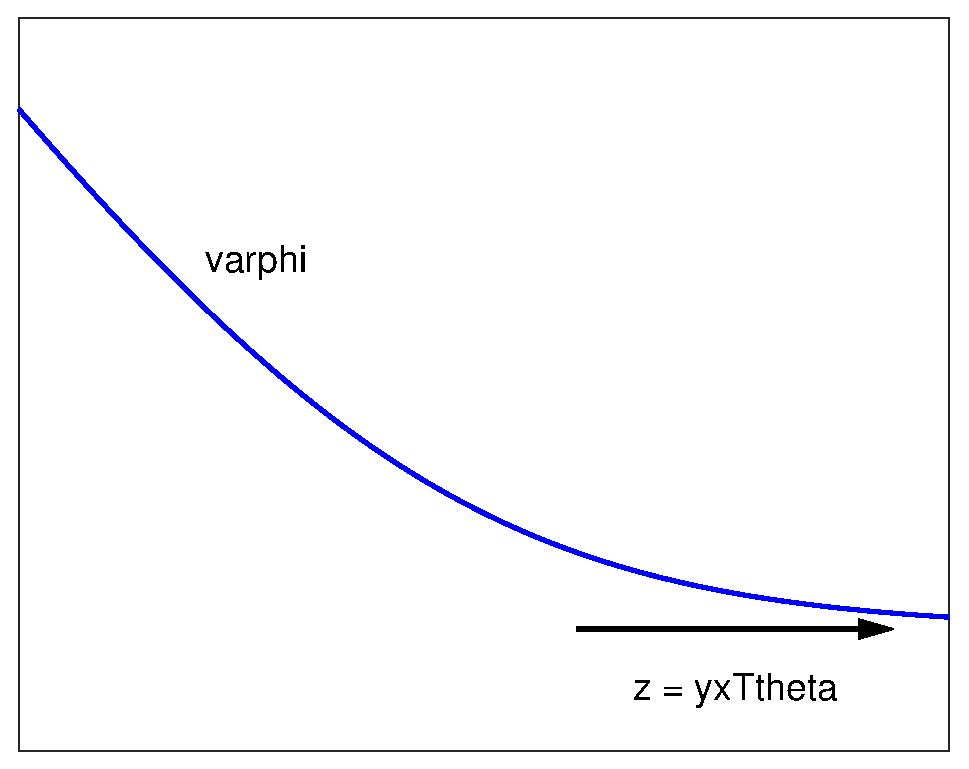
\includegraphics[width=.6\columnwidth]{logistic-loss.eps}
    \caption{\label{fig:simple-loss-shape} The rough shape
      of loss we desire: the loss is convex and continuous,
      and tends to zero as the margin $z = y x^T \theta \to \infty$.}
  \end{center}
\end{figure}
That is, we will essentially always use losses that satisfy
\begin{equation*}
  \loss(z) \to 0
  ~~ \mbox{as}~ z \to \infty,
  ~~ \mbox{while} ~~
  \loss(z) \to \infty
  ~~ \mbox{as} ~ z \to -\infty.
\end{equation*}

As a few different examples, here are three loss functions that
we will see either now or later in the class, all of which are commonly
used in machine learning.
\begin{enumerate}[(i)]
\item The \emph{logistic loss} uses
  \begin{equation*}
    \logloss(z) = \log(1 + e^{-z})
  \end{equation*}
\item The \emph{hinge loss} uses
  \begin{equation*}
    \hingeloss(z) = \hinge{1 - z}
    = \max\{1 - z, 0\}
  \end{equation*}
\item The \emph{exponential loss} uses
  \begin{equation*}
    \exploss(z) = e^{-z}.
  \end{equation*}
\end{enumerate}
In Figure~\ref{fig:loss-functions}, we plot each of these losses
against the margin $z = y x^T \theta$, noting that each goes to zero
as the margin grows, and each tends to $+\infty$ as the margin becomes
negative. The different loss functions lead to different machine
learning procedures; in particular, the logistic loss
$\logloss$ is logistic regression, the
hinge loss $\hingeloss$ gives rise to so-called \emph{support vector
machines}, and the exponential loss gives rise to the classical
version of \emph{boosting}, both of which we will explore in more depth
later in the class.

\begin{figure}[h!]
  \begin{center}
    \psfrag{Logistic}{$\logloss$}
    \psfrag{Hinge}{$\hingeloss$}
    \psfrag{Exp}{$\exploss$}
    \psfrag{z = yxTtheta}{$z = y x^T \theta$}
    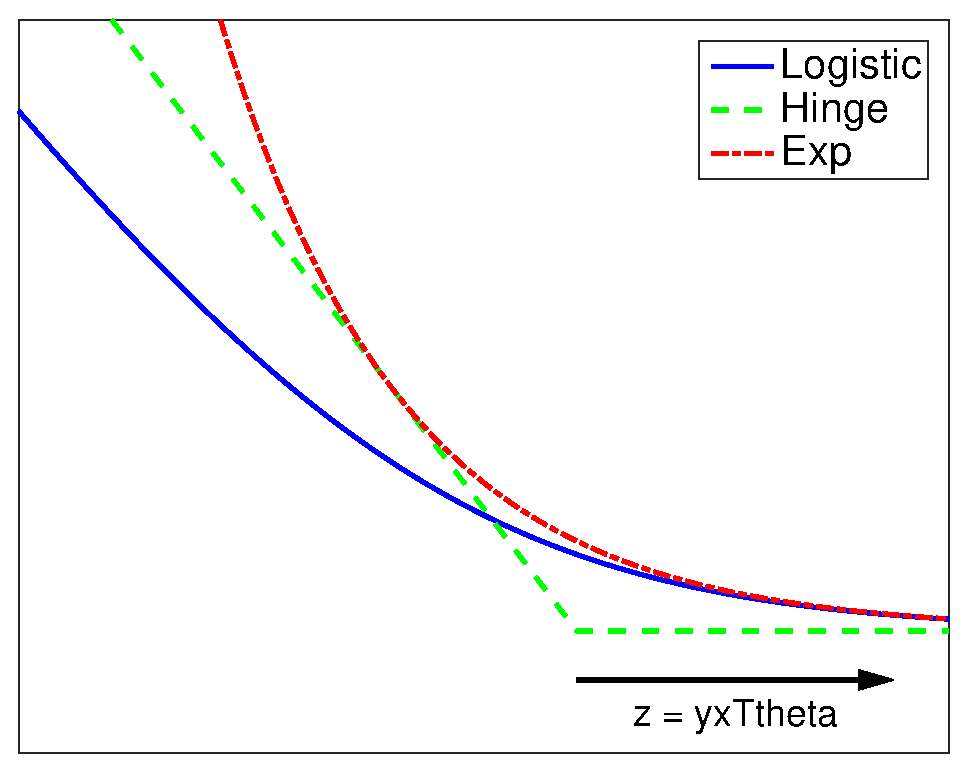
\includegraphics[width=.7\columnwidth]{many-losses.eps}
    \caption{\label{fig:loss-functions} The three margin-based loss
      functions logistic loss, hinge loss, and exponential loss.}
  \end{center}
\end{figure}

\section{Logistic regression}

With this general background in place, we now we give a complementary view
of logistic regression to that in Andrew Ng's lecture notes.
When we use binary labels $y \in \{-1, 1\}$, it is possible to
write logistic regression more compactly. In particular, we use the
logistic loss
\begin{equation*}
  \logloss(y x^T\theta)
  = \log\left(1 + \exp(-y x^T \theta)\right),
\end{equation*}
and the \emph{logistic regression} algorithm corresponds to choosing
$\theta$ that minimizes
\begin{equation}
  \label{eqn:logreg-risk}
  J(\theta) = \frac{1}{m}
  \sum_{i=1}^m \logloss(\ysi \theta^T \xsi)
  = \frac{1}{m} \sum_{i=1}^m \log\left(1 + \exp(-\ysi \theta^T \xsi)\right).
\end{equation}
Roughly, we hope that choosing $\theta$ to minimize the average logistic
loss will yield a $\theta$ for which $\ysi \theta^T \xsi > 0$ for most (or
even all!) of the training examples.


\subsection{Probabilistic intrepretation}

\begin{figure}[ht]
  \begin{center}
    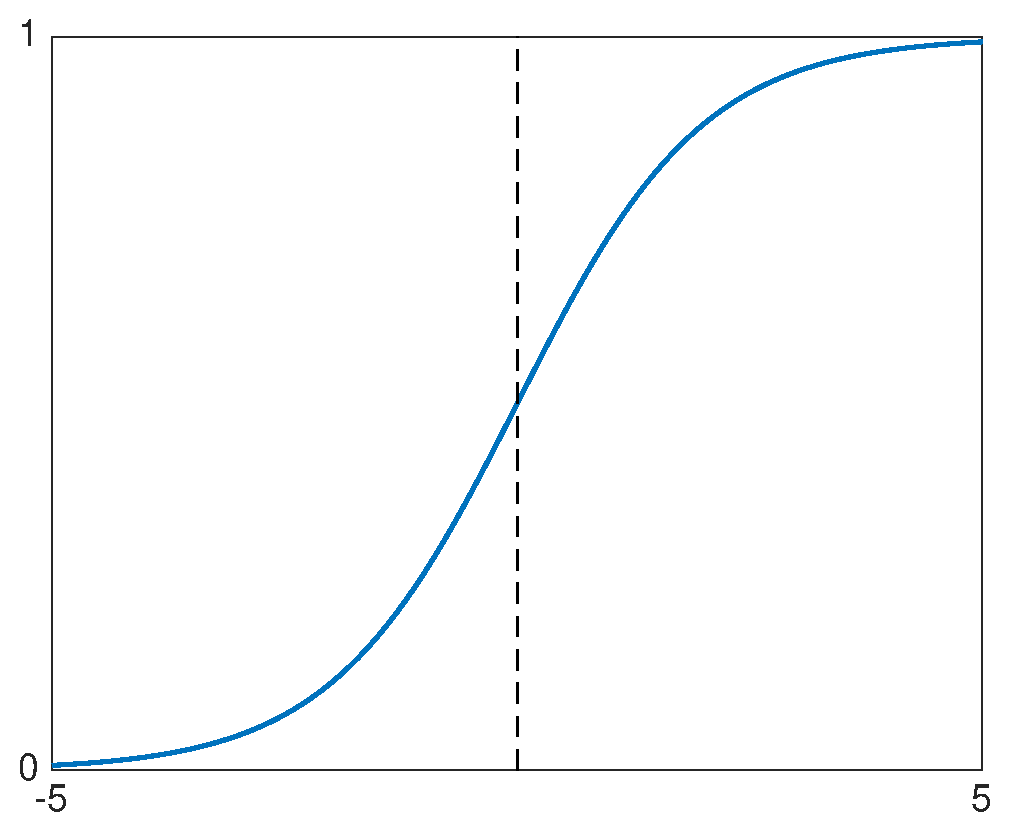
\includegraphics[width=.6\columnwidth]{sigmoid.eps}
    \caption{\label{fig:sigmoid} Sigmoid function}
  \end{center}
\end{figure}

Similar to the linear regression (least-squares) case, it
is possible to give a probabilistic interpretation of logistic
regression. To do this, we define the \emph{sigmoid function}
(also often called the \emph{logistic function})
\begin{equation*}
  g(z) = \frac{1}{1 + e^{-z}},
\end{equation*}
which is plotted in Fig.~\ref{fig:sigmoid}. In particular,
the sigmoid function satisfies
\begin{equation*}
  g(z) + g(-z) = \frac{1}{1 + e^{-z}} + \frac{1}{1 + e^z}
  = \frac{e^z}{1 + e^z} + \frac{1}{1 + e^z} = 1,
\end{equation*}
so we can use it to define a probability model for binary classification.
In particular, for $y \in \{-1, 1\}$, we define the \emph{logistic
model} for classification as
\begin{equation}
  \label{eqn:logistic-model}
  p(Y = y \mid x; \theta)
  = g(y x^T \theta)
  = \frac{1}{1 + e^{-y x^T \theta}}.
\end{equation}
For intepretation, we see that if the margin
$y x^T \theta$ is large---bigger than, say, 5 or so---then
$p(Y = y \mid x; \theta) = g(y x^T \theta) \approx 1$, that is, 
we assign nearly probability $1$ to the event that the label is $y$.
Conversely, if $y x^T \theta$ is quite negative, then
$p(Y = y \mid x; \theta) \approx 0$.

By redefining our hypothesis class as
\begin{equation*}
  h_\theta(x) = g(\theta^T x) = \frac{1}{1 + e^{-\theta^T x}},
\end{equation*}
then we see that the likelihood of the training data is
\begin{equation*}
  L(\theta)
  = \prod_{i = 1}^m p(Y = \ysi \mid \xsi; \theta)
  = \prod_{i = 1}^m h_\theta(\ysi \xsi),
\end{equation*}
and the log-likelihood is precisely
\begin{equation*}
  \ell(\theta)
  = \sum_{i = 1}^m \log h_\theta(\ysi \xsi)
  = -\sum_{i = 1}^m \log\left(1 + e^{-\ysi \theta^T \xsi}\right)
  = - m J(\theta),
\end{equation*}
where $J(\theta)$ is exactly the logistic regression
risk from Eq.~\eqref{eqn:logreg-risk}. That is, maximum likelihood
in the logistic model~\eqref{eqn:logistic-model} is the same
as minimizing the average logistic loss, and we arrive at logistic
regression again.

\subsection{Gradient descent methods}

The final part of logistic regression is to actually fit the model.
As is usually the case, we consider gradient-descent-based procedures
for performing this minimization. With that in mind, we now show
how to take derivatives of the logistic loss.
For $\logloss(z) = \log(1 + e^{-z})$,
we have the one-dimensional derivative
\begin{equation*}
  \frac{d}{dz} \logloss(z)
  = \logloss'(z)
  = \frac{1}{1 + e^{-z}} \cdot \frac{d}{dz} e^{-z}
  = -\frac{e^{-z}}{1 + e^{-z}}
  = - \frac{1}{1 + e^z} = - g(-z),
\end{equation*}
where $g$ is the sigmoid function. Then we apply the chain rule to find that
for a single training example $(x, y)$, we have
\begin{equation*}
  \frac{\partial}{\partial \theta_k}
  \logloss(y x^T \theta)
  = -g(-y x^T \theta) \frac{\partial}{\partial \theta_k} (y x^T \theta)
  = -g(-y x^T\theta) y x_k.
\end{equation*}
Thus, a stochastic gradient procedure for minimization of $J(\theta)$
iteratively performs the following for iterations
$t = 1, 2, \ldots$, where $\stepsize_t$ is a stepsize at time $t$:
\begin{enumerate}[1.]
\item Choose an example $i \in \{1, \ldots, m\}$ uniformly at random
\item Perform the gradient update
  \begin{align*}
    \theta^{(t + 1)}
    & = \theta^{(t)}
    - \stepsize_t \cdot \nabla_\theta \logloss(\ysi \xsi^T \theta^{(t)}) \\
    & = \theta^{(t)}
    + \stepsize_t
    g(-\ysi \xsi^T \theta^{(t)}) \ysi \xsi
    = \theta^{(t)}
    + \stepsize_t
    h_{\theta^{(t)}} (-\ysi \xsi) \ysi \xsi.
  \end{align*}
\end{enumerate}
This update is intuitive: if our current hypothesis
$h_{\theta^{(t)}}$ assigns probability close to $1$ for the
\emph{incorrect} label $-\ysi$, then we try to reduce the loss
by moving $\theta$ in the direction of $\ysi \xsi$. Conversely,
if our current hypothesis $h_{\theta^{(t)}}$ assigns probability
close to $0$ for the incorrect label $-\ysi$, the update essentially
does nothing.


\end{document}
